\section{Đề xuất phát triển}

\subsection{Chiến lược khai phá đặc trưng dựa trên độ trùng lắp}
Ảnh tham khảo truy xuất được từ tác vụ VPR tiềm ẩn rủi ro không đủ độ trùng lắp với ảnh đầu vào, dẫn đến sai sót trong quá trình tính toán tư thế. Để giải quyết vấn đề này, chúng tôi đề xuất một chiến lược khai phá mới dựa trên hàm khai phá Multi-Similarity Miner \cite{wang2019multi} nhằm đảm bảo tính trùng lấp về vùng khung hình(frustum) cao giữa các ảnh. Điều này sẽ hỗ trợ cho quá trình Feature Matching tại module RPR ở phía sau.

Cụ thể hơn, chúng tôi xác định một cặp ảnh là được một positive pair nếu có độ trùng lắp frustum cao hơn một ngưỡng nhất định, tức giữa cặp ảnh chia sẻ nhiều điểm chung hơn. Để đảm bảo độ vững chắc của mô hình không bị tác động, chúng tôi sử dụng cơ chế trùng lắp camera frustum song phương từ \cite{9008579}, được tính bằng tổng độ trùng lắp frustum từ một ảnh đến ảnh còn lại và ngược lại.

Tuy nhiên, độ trùng lắp cao vẫn có thể xuất hiện trong trường hợp các ảnh được chụp ở hai góc độ hoàn toàn ngược nhau, gây nên khó khăn và sai lệch trong quá trình dự đoán tư thế tuyệt đối do góc quay khác biệt quá lớn. Để giải quyết vấn đề này, chúng tôi đặt ra điều kiện khác biệt hướng nhìn làm một tiêu chuẩn phụ trong việc chấp nhận các cặp ảnh. Cụ thể hơn, các cặp ảnh không được phép có hướng nhìn lệch nhau quá một tiêu chuẩn nhất định mà chúng tôi đặt ra.

% \begin{figure}
%   \centering
%   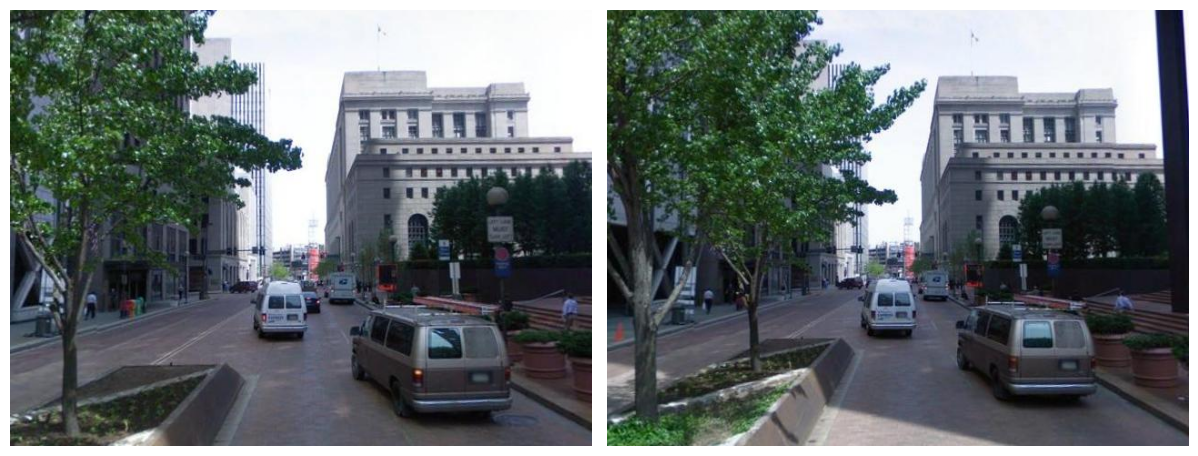
\includegraphics[width=\textwidth]{pics/Chapter3/highoverlap.png}
%   \caption[Cặp ảnh có độ overlap cao]{Cặp ảnh được chấp nhận - có độ trùng lắp cao}
% \end{figure}

% \begin{figure}
%   \centering
%   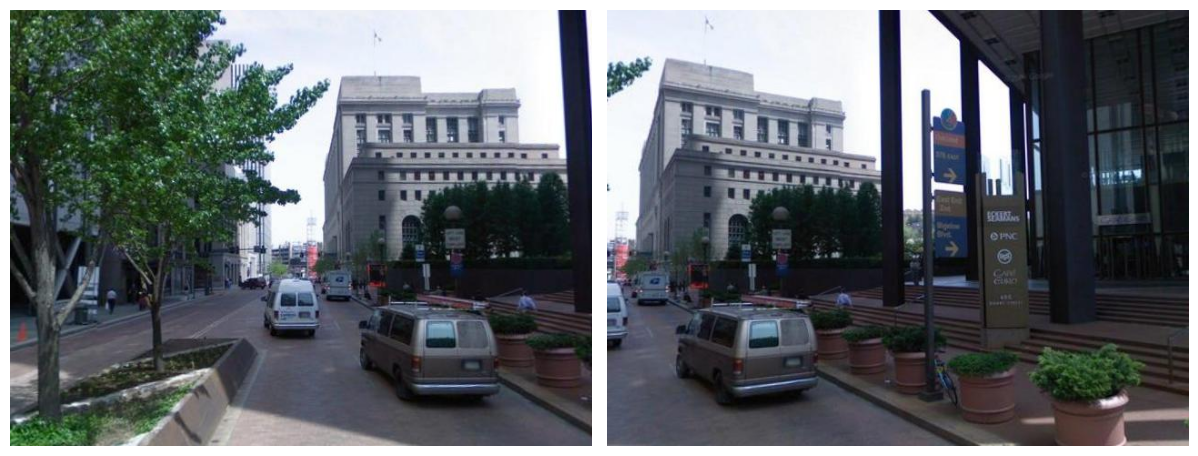
\includegraphics[width=\textwidth]{pics/Chapter3/lowoverlap.png}
%   \caption[Cặp ảnh có độ overlap thấp]{Cặp ảnh không được chấp nhận - có độ trùng lắp thấp}
% \end{figure}

\begin{figure}
  \centering
  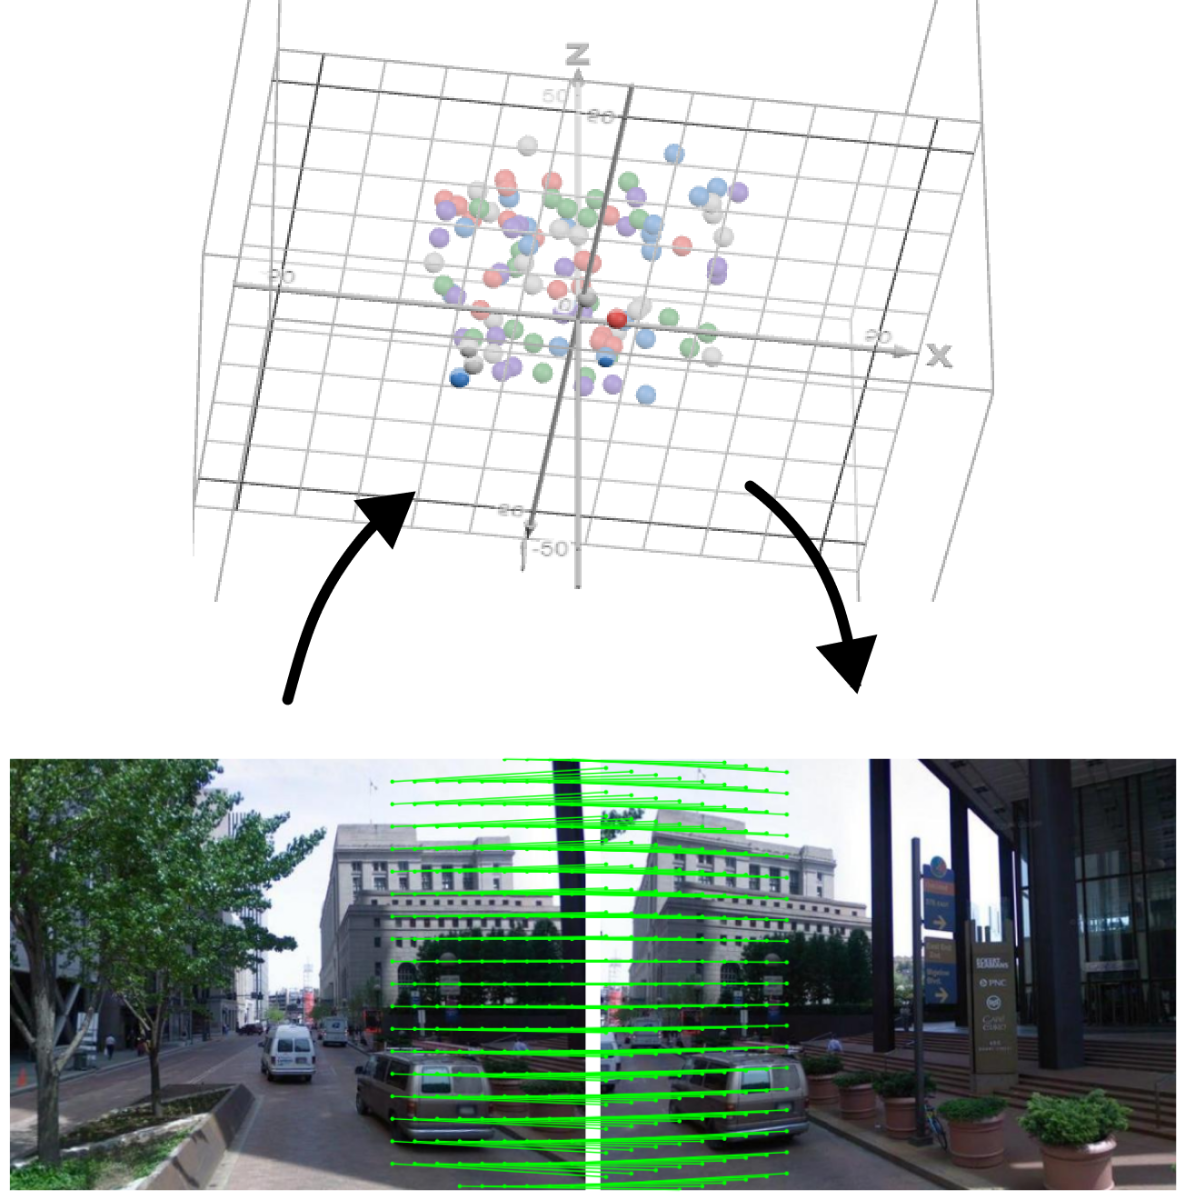
\includegraphics[width=0.6\textwidth]{pics/Proposal/project.drawio.png}
  \caption[Quá trình chiếu giữa 2 ảnh]{Ảnh mô tả quá trình chiếu từ ảnh đầu tiên lên không gian 3D rồi back-project lên không gian khung hình của ảnh thứ 2}
\end{figure}

\subsubsection*{Độ trùng lắp Frustum}

Độ trùng lắp frustum giữa hai ảnh có thể được định nghĩa là tổng tỷ lệ các điểm ảnh thuộc ảnh thứ nhất nằm trong vùng tầm nhìn khi chiếu lên hệ tọa độ camera thứ hai, và ngược lại. Độ trùng lắp này được tính toán bằng cách trước hết chiếu các điểm ảnh từ hình ảnh gốc vào không gian 3D thông qua việc tận dụng độ sâu ước lượng được. Sau đó, các điểm ảnh này được chiếu vào hệ tọa độ của hình ảnh thứ hai bằng cách tận dụng thông tin vị trí và góc quay của chúng.

Đầu tiên, một ma trận các điểm ảnh với kích thước 10x10 được chiếu vào hệ tọa độ thực, sau đó lại được chiếu lại vào hệ tọa độ camera thứ hai. Phép chiếu có thể được công thức hóa như sau:
$$
W = R_1\cdot \left[(K_1^{-1} \cdot P_1)*D_1(P_1)\right] + t_1
$$

$$
P_2 = K_2 \cdot\left[R_2^{T} \cdot (W - t_2)\right]
$$
với $P_i$ là vị trí điểm ảnh trong camera $i$, $K_i$ là ma trận intrinsics, $R_i$ và $t_i$ là độ lệch góc quay và vị trí từ hệ tọa độ camera sang hệ tọa độ thực với $R$ là vector góc quay thu được từ quaternion tương ứng, và $D_i(P)$ là ước lượng độ sâu theo đơn vị khoảng cách của điểm ảnh $P$.

\subsubsection*{Khác biệt hướng nhìn}

Để kiểm soát cách biệt góc quay giữa hai ảnh, chúng tôi đo độ cách biệt về hướng nhìn giữa chúng. Độ lệch góc quay camera $\alpha$ giữa hai camera có thể được định nghĩa như sau:

$$
\alpha = arccos\left(\frac{trace(R_1^T \cdot R_2 - 1)}{2} \right) / \pi * 180
$$

với $\alpha$ mang đơn vị độ và $R_i$ là ma trận 3x3 thể hiện góc quay của ảnh.

\subsubsection*{Hàm Loss}

Hàm loss của chúng tôi được tính toán bằng tổng có trọng số giữa hai hàm loss với một biến số 'Control Rate' - tỷ lệ kiểm soát:
$$
L = \beta * L_{Miner} + (1-\beta)*L_{Control}
$$
với $L_{Control}$ là hàm Multi-Similarity Loss từ bài báo Multi-Similarity Miner và $L_{Miner}$ là hàm Multi-Similarity Loss nhận đầu ra từ chiến lược khai phá frustum mới của chúng tôi và $\beta$ là giá trị tỷ lệ để kiểm soát hai hàm Loss trên.

\subsection{Chiến lược sắp xếp lại ảnh}
Một số nghiên cứu trước đây đã thiết kế tác vụ truy xuất ảnh ở module VPR thành một quá trình gồm 2 bước đi từ kết quả thô đến kết quả chính xác. Việc thực hiện quá trình 2 bước này giúp cho mô hình VPR có thể lọc được tập kết quả thô ban đầu và sau đó tinh chỉnh lại xếp hạng của các kết quả theo một tiêu chí khác. Trong phương pháp đề xuất của chúng tôi, bước truy xuất đầu tiên sẽ được dùng để xác định một tập $k_1$ các ảnh được chụp gần với ảnh truy vấn. Sau đó, bước sắp xếp lại phía sau sẽ sắp xếp lại thứ tự ảnh, sắp xếp theo ưu tiên những ảnh có độ trùng lấp cao với ảnh truy vấn và xác định top $k_2$ ảnh có độ trùng lấp cao nhất.

Với bước truy xuất ban đầu, chúng tôi sử dụng trọng số baseline được cung cấp bởi mô hình MixVPR, do đã được chứng minh là có hiệu quả tốt trong việc xác định ảnh tham khảo có vị trí gần với ảnh truy vấn. Sau đó, ở bước sắp xếp lại thứ tự, chúng tôi sử dụng một trọng số khác của MixVPR đã được huấn luyện lại, tập trung vào việc xác định những ảnh có độ trùng lấp cao với nhau. 

Để có được trọng số mới, chúng tôi huấn luyện mô hình trên tập dữ liệu GSV-Cities \cite{Ali_bey_2022} với mỗi batch sẽ chỉ gồm các ảnh từ 1 khu vực. Mô hình sẽ tập trung vào việc phân biệt những ảnh có độ trùng lấp khung hình cao và thấp theo tiêu chí đã được đặt ra ở \textbf{3.4.1}.

\begin{figure}
  \centering
  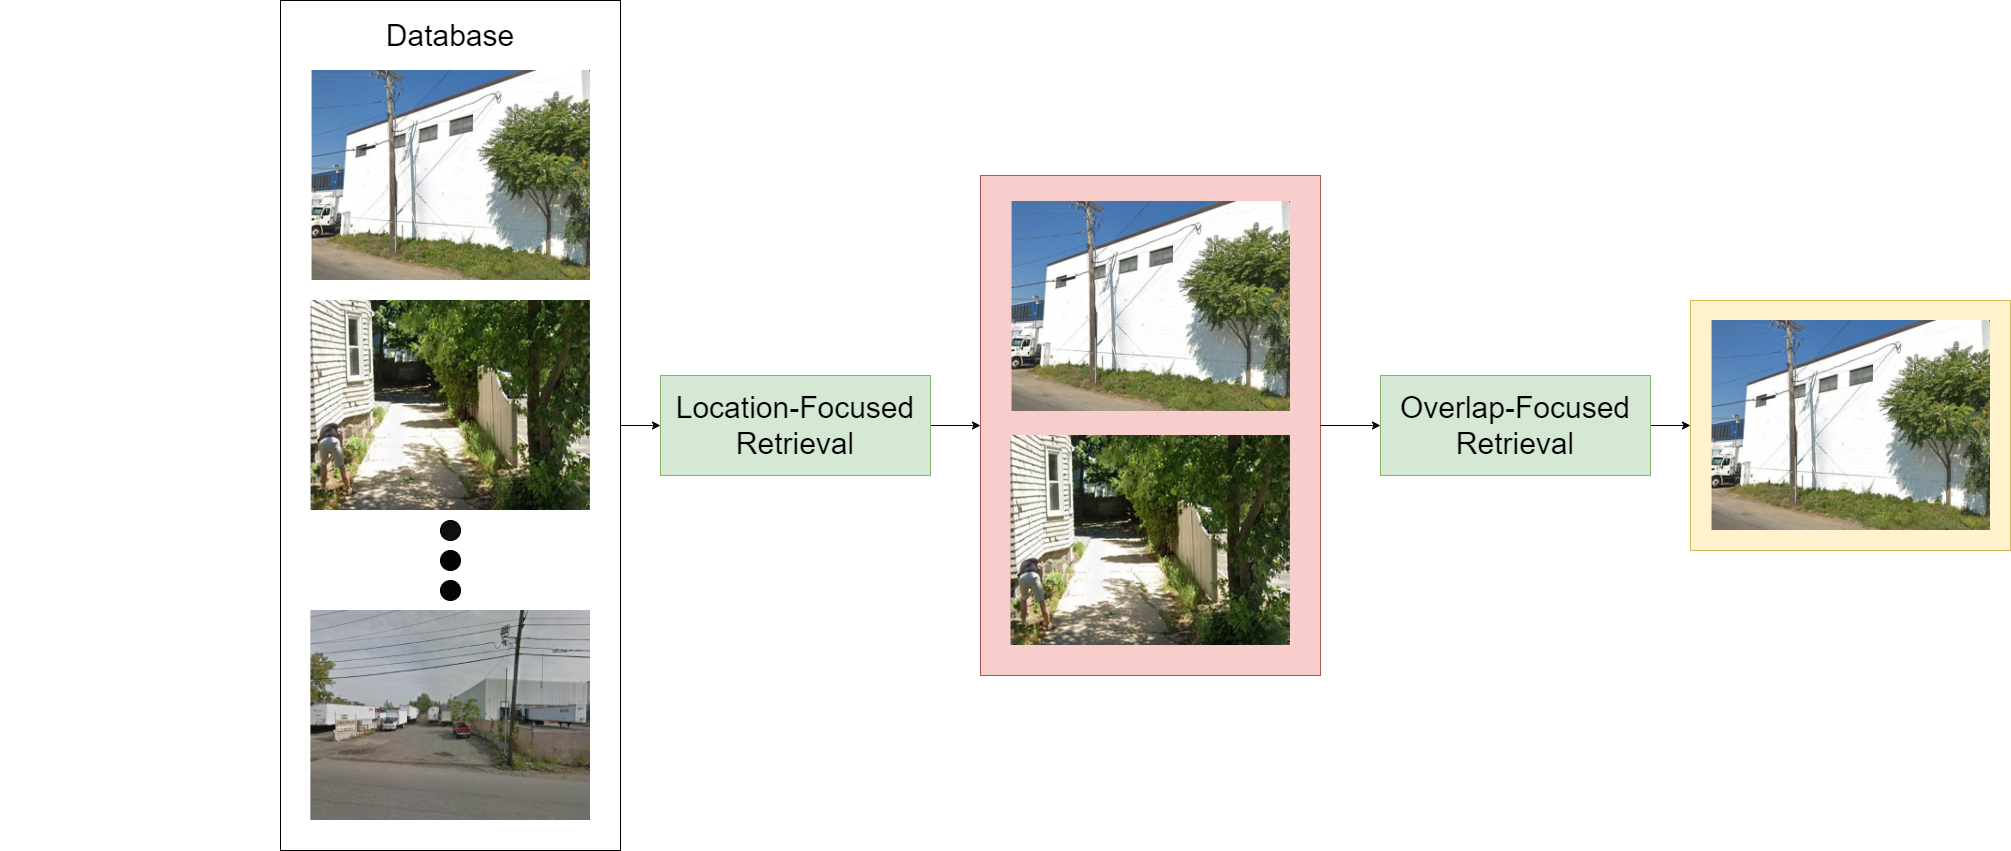
\includegraphics[width=\textwidth]{pics/Proposal/rerank.drawio.png}
  \caption[Quá trình truy xuất 2 bước của VPR]{Quá trình truy xuất gồm 2 bước của mô hình VPR, gồm truy xuất theo địa điểm và truy xuất theo độ trùng lắp}
\end{figure}

\subsection{Trung bình trọng số của các dự đoán}

Ở pipeline cơ bản được đề xuất của nhóm, module VPR sẽ truy xuất được $k$ ảnh tham khảo và từ đó có thể xác định được $k$ dự đoán khác nhau tương ứng với mỗi ảnh. Kết quả cuối cùng sẽ là dự đoán có độ đáng tin cậy $C$ cao nhất. Tuy nhiên, khi chọn theo cơ chế tối đa như thế, thông tin lấy được từ những dự đoán của những ảnh còn lại sẽ bị lãng phí. Vì vậy nên, chúng tôi giới thiệu phương pháp lấy trung bình của từng dự đoán dựa vào với trọng số tương ứng với độ đáng tin $C$.

\begin{figure}[H]
  \centering
  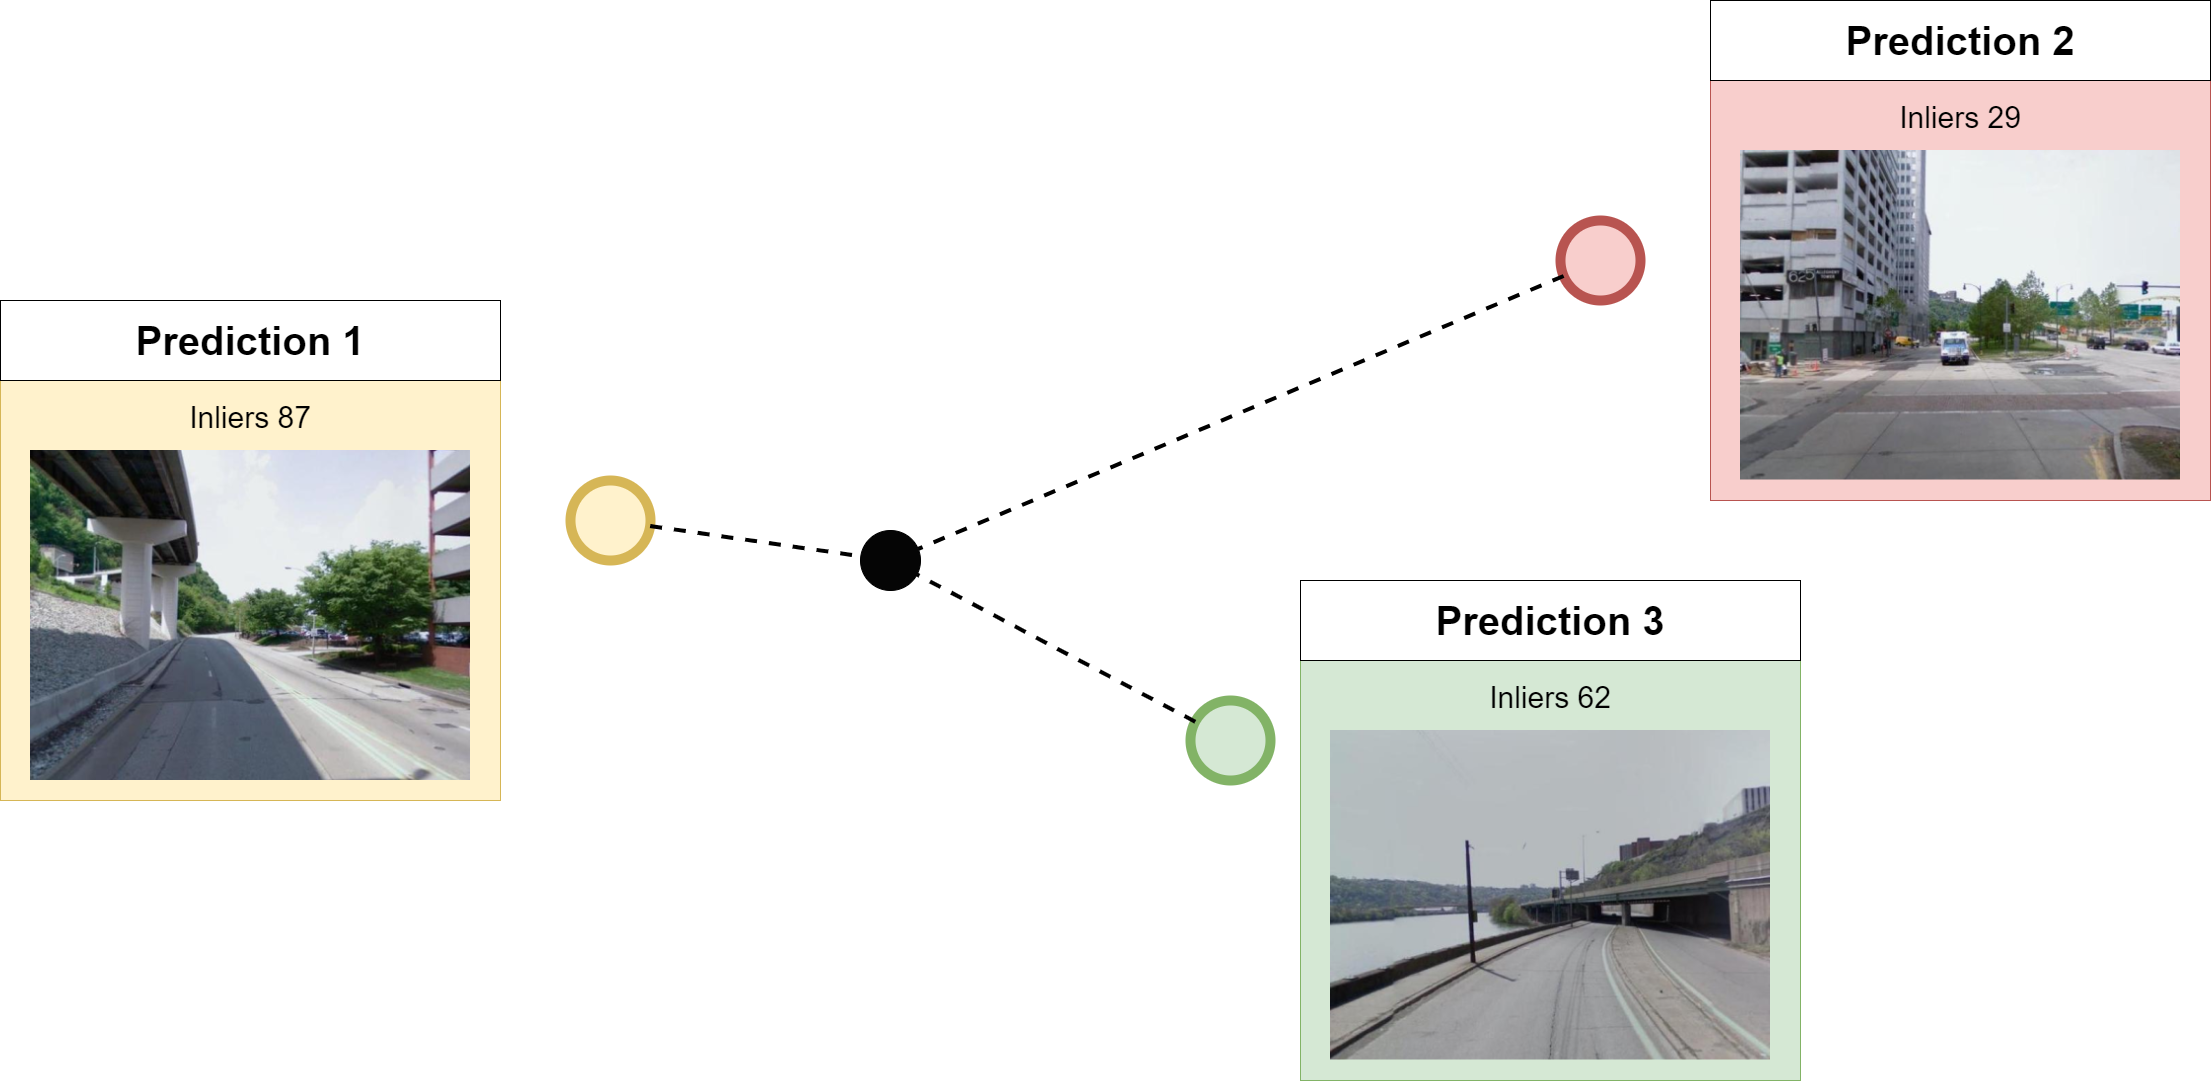
\includegraphics[width=\textwidth]{pics/Proposal/weighted.png}
  \caption[Trung bình trọng số theo inliers của dự đoán]{Mô tả phương pháp lấy trung bình trọng số của các dự đoán theo độ tin cậy của dự đoán}
\end{figure}

\subsection{Giới hạn ngưỡng đáng tin của kết quả}

Độ đáng tin cậy $C$ của dự đoán của cặp ảnh truy vấn và tham khảo được định nghĩa là số cặp điểm tương quan giữa hai hình mà khi áp dụng phép biến đổi tương ứng với độ lệch về tư thế giữa hai ảnh, cho ra độ lệch dưới một ngưỡng nhất định. Càng nhiều điểm thỏa được phép biến đổi thì cơ sở để suy luận ra được độ lệch giữa hai ảnh càng thêm chắc chắn. Vì vậy nên, để đảm bảo được dự đoán của pipeline có thể được tin tưởng, chúng tôi áp dụng một bước lọc lại dự đoán ở cuối pipeline, nhằm lọc ra những kết quả có độ đáng tin cậy thấp, từ đó cải thiện hiệu quả của mô hình.

\begin{figure}[H]
  \centering
  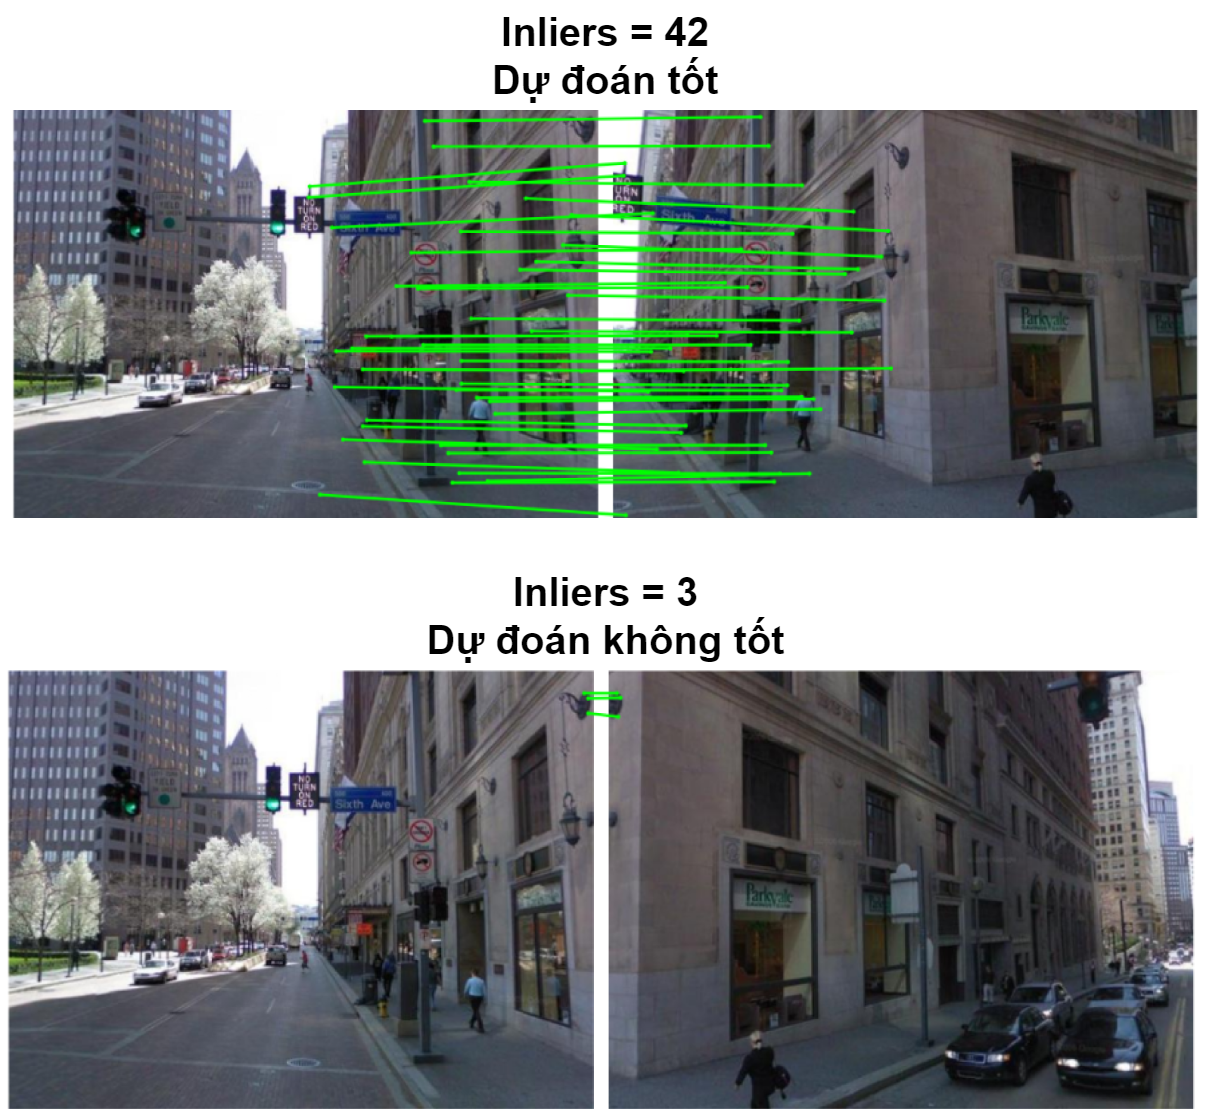
\includegraphics[width=0.75\textwidth]{pics/Proposal/threshold.png}
  \caption[Những dự đoán tốt và không tốt đánh giá theo độ tin cậy]{Mô tả những trường hợp có độ tự tin cao và thấp trong tập dữ liệu Pittsburgh250k \cite{6618963}}
\end{figure}

